\documentclass[aspectratio=169,10pt]{beamer}
\usetheme{metropolis}
\usepackage{amsmath,amssymb,bm,booktabs,xcolor}
\usepackage{tikz}
\usepackage{graphicx}
\usetikzlibrary{arrows.meta,positioning,fit,backgrounds}

\title{Controlling Cup-Ball:\\How the Body Helps the Brain}
\subtitle{}
\author{Meeting Notes --- March 2026, Dipankar Bhattacharya}
\date{}

% ── colour helpers ────────────────────────────────────────────────────────────
\definecolor{mgreen}{RGB}{30,140,60}
\definecolor{morange}{RGB}{210,110,0}

\begin{document}

% ── Title ─────────────────────────────────────────────────────────────────────
\maketitle

% ── Slide 1: The shared task ────────────────────────────────────────────────
\begin{frame}{The Shared Experimental Platform}
\begin{columns}[T]
  \column{0.55\textwidth}
  \textbf{Task:} transport a cup of coffee (Cup-ball (cart-pendulam) proxy) along a
  horizontal track using a haptic manipulandum.\\[6pt]
  \textbf{Challenge:} the pendulum is \emph{unactuated}---the brain controls
  only the cup position, not the ball inside.\\[6pt]
  \textbf{Probe:} impulsive perturbations (assistive / resistive / unexpected)
  are injected mid-motion to reveal the control strategy.\\[6pt]
  \textbf{Why it matters:} mirrors everyday manipulation of underactuated
  objects (cups, tools, bags).

  \column{0.42\textwidth}
  \begin{block}{Three papers, one platform}
    \begin{itemize}\setlength\itemsep{4pt}
      \item \textbf{Bazzi 2018} --- stability analysis
      \item \textbf{Razavian 2021} --- zero-force trajectory
      \item \textbf{Razavian 2023} --- body mechanics + OFC
    \end{itemize}
  \end{block}
  \vspace{4pt}
  Each paper probes a \emph{different} facet of the same question:\\
  \emph{How do humans tame complex internal dynamics?}
\end{columns}
\end{frame}

% ── Slide 2: Bazzi 2018 ─────────────────────────────────────────────────────
\begin{frame}{Paper 1 · Bazzi et al.\ 2018 --- Exploiting Passive Contraction}
\begin{columns}[T]
  \column{0.55\textwidth}
  \textbf{Core idea:} identify regions of state space where the cart--pendulum
  dynamics are \emph{self-converging} (contraction regions), then test whether
  humans steer through them.\\[5pt]
  \textbf{Why not Lyapunov?}  Lyapunov requires proximity to a fixed
  equilibrium.  Transport tasks begin and end \emph{far} from equilibrium
  $\Rightarrow$ contraction analysis is the right tool.\\[5pt]
  \textbf{Key findings:}
  \begin{itemize}\setlength\itemsep{3pt}
    \item \textcolor{mgreen}{Assistive} perturbation --- trajectories enter
          a contraction region \emph{before} the perturbation; convergent
          dynamics absorb the disturbance.
    \item \textcolor{morange}{Resistive} perturbation --- trajectories enter
          a contraction region only \emph{after} the perturbation (reactive
          re-stabilisation).
    \item Humans did \textbf{not} minimise force.  Two prior studies showed
          subjects \textbf{maximised predictability} measured by
          \emph{mutual information} --- not energy or force.
  \end{itemize}

  \column{0.42\textwidth}
  \begin{alertblock}{Take-home}
    Humans exploit the \emph{task's own dynamics} to stabilise movement.
    By traversing contraction regions they avoid chaotic amplification of
    errors and make their behaviour \emph{more predictable} --- without
    needing to minimise force or compute an optimal trajectory.
  \end{alertblock}
  \vspace{5pt}
  \begin{block}{What it does NOT provide}
    \begin{itemize}\setlength\itemsep{2pt}
      \item No explicit controller model
      \item No cost function
    \end{itemize}
  \end{block}
\end{columns}
\end{frame}

% ── Slide 3: Razavian 2021 ──────────────────────────────────────────────────
\begin{frame}{Paper 2 · Razavian et al.\ 2021 --- The Zero-Force Trajectory}
\begin{columns}[T]
  \column{0.55\textwidth}
  \textbf{Problem:} standard models (min-jerk, OFC min-effort, constant
  impedance) all fail when real cup-and-ball dynamics are present.\\[6pt]
  \textbf{Proposed solution --- three elements combined:}
  \begin{enumerate}\setlength\itemsep{3pt}
    \item Spring--damper \textbf{impedance} between OFC reference and cup.
    \item \textbf{OFC} in the feedback loop (not a pre-planned trajectory).
    \item \textbf{Minimum-jerk} objective.
  \end{enumerate}
  \vspace{4pt}
  \textbf{Zero-force trajectory:}  The smooth, jerk-minimising OFC reference
  $y_\text{ref}(t)$ keeps the impedance from pushing against the pendulum
  --- it is \emph{not} obtained by minimising $F_\text{inter}$ directly.

  \column{0.42\textwidth}
  \begin{alertblock}{Take-home}
    Impedance + OFC + minimum jerk is the \emph{minimal} combination
    that reproduces human cup-and-ball behaviour.\\[4pt]
    No single element alone is sufficient.
  \end{alertblock}
  \vspace{6pt}
  Signal chain:\vspace{2pt}
  \[
    u \xrightarrow{\tau_m} F \xrightarrow{M_\text{ref}} y_\text{ref}
      \xrightarrow{k,d} F_\text{imp} \to \text{plant}
  \]
\end{columns}
\end{frame}

% ── Slide 4: Razavian 2023 ──────────────────────────────────────────────────
\begin{frame}{Paper 3 · Razavian et al.\ 2023 --- Body Mechanics Subsumes Control}
\begin{columns}[T]
  \column{0.55\textwidth}
  \textbf{Question:} if we add mechanical impedance to the body model, what
  can we still infer about the neural controller?\\[4pt]
  \textbf{Four OFC variants:} min-effort vs.\ min-jerk $\times$ with vs.\
  without impedance.\\[4pt]
  \textbf{Three key findings:}
  \begin{enumerate}\setlength\itemsep{2pt}
    \item \textbf{Impedance is essential.}  Reproduces force jump \&
          velocity rebound ${<}20$\,ms --- faster than any reflex.
    \item \textbf{Cost function irrelevant.}  With impedance, effort and
          jerk models fit equally well ($p \geq 0.195$).
    \item \textbf{Feedback $\equiv$ feedforward.}  Impedance handles
          catch trials; online feedback adds nothing.
  \end{enumerate}

  \column{0.42\textwidth}
  \begin{alertblock}{Take-home}
    Ignoring impedance \emph{over-credits the brain}.\\[4pt]
    The arm's passive spring--damper mechanics produce rapid disturbance
    rejection and make different ``optimal'' strategies look
    indistinguishable in the data.
  \end{alertblock}
\end{columns}
\end{frame}

% ── Slide 5: Side-by-side comparison ────────────────────────────────────────
\begin{frame}{Side-by-Side Comparison}
\begin{center}
\small
\begin{tabular}{@{}lp{3.0cm}p{3.0cm}p{3.2cm}@{}}
\toprule
 & \textbf{Bazzi 2018} & \textbf{Razavian 2021} & \textbf{Razavian 2023} \\
\midrule
\textbf{Core tool}       & Contraction / PDE metric & Impedance-mediated OFC & Stochastic OFC + impedance \\
\textbf{Controller?}     & None (analysis only)     & Partial (impedance attractor) & Full LQG + muscle \\
\textbf{Cost function}   & N/A                     & Min jerk $\Rightarrow$ ZFT   & Effort vs.\ jerk --- indistinguishable \\
\textbf{Feedback role}   & Bypassed by contraction  & Not analysed            & Redundant when impedance present \\
\textbf{Main finding}    & Humans exploit passive convergence & ZFT is key reference & Body mechanics subsumes controller \\
\bottomrule
\end{tabular}
\end{center}

\vspace{6pt}
\begin{block}{Common thread}
  All three papers show that \emph{passive body mechanics} --- not neural
  computation alone --- are the decisive factor in successful
  complex-object manipulation.
\end{block}
\end{frame}

% ── Slide 6: Implications for our project ───────────────────────────────────
\begin{frame}{Implications for Our Project}
\begin{columns}[T]
  \column{0.5\textwidth}
  \textbf{What we need (and have):}
  \begin{itemize}\setlength\itemsep{5pt}
    \item[\textcolor{mgreen}{\checkmark}] Impedance controller
          $F_\text{imp}=K\Delta p + D\Delta\dot{p}$
    \item[\textcolor{mgreen}{\checkmark}] ZFT reference mass block
    \item[\textcolor{mgreen}{\checkmark}] LQR + muscle dynamics (14-D state)
    \item[\textcolor{mgreen}{\checkmark}] Cart-pendulum PyDrake simulation
  \end{itemize}

  \column{0.47\textwidth}
  \textbf{What we do NOT need (for now):}
  \begin{itemize}\setlength\itemsep{5pt}
    \item[\textcolor{morange}{$\times$}] Contraction theory
          --- useful for analysis, not for building the controller
    \item[\textcolor{morange}{$\times$}] Exhaustive cost-function comparison
          --- with impedance, both objectives perform the same
  \end{itemize}
\end{columns}
\vspace{10pt}
\begin{alertblock}{Bottom line}
  Impedance is the critical architectural ingredient.  The LQR / OFC choice
  and feedback structure are secondary once impedance is in the loop.
\end{alertblock}
\end{frame}

% ── Slide 7: Our Implementation Architecture ────────────────────────────────
\begin{frame}{Our Implementation: System Architecture}
\begin{center}
  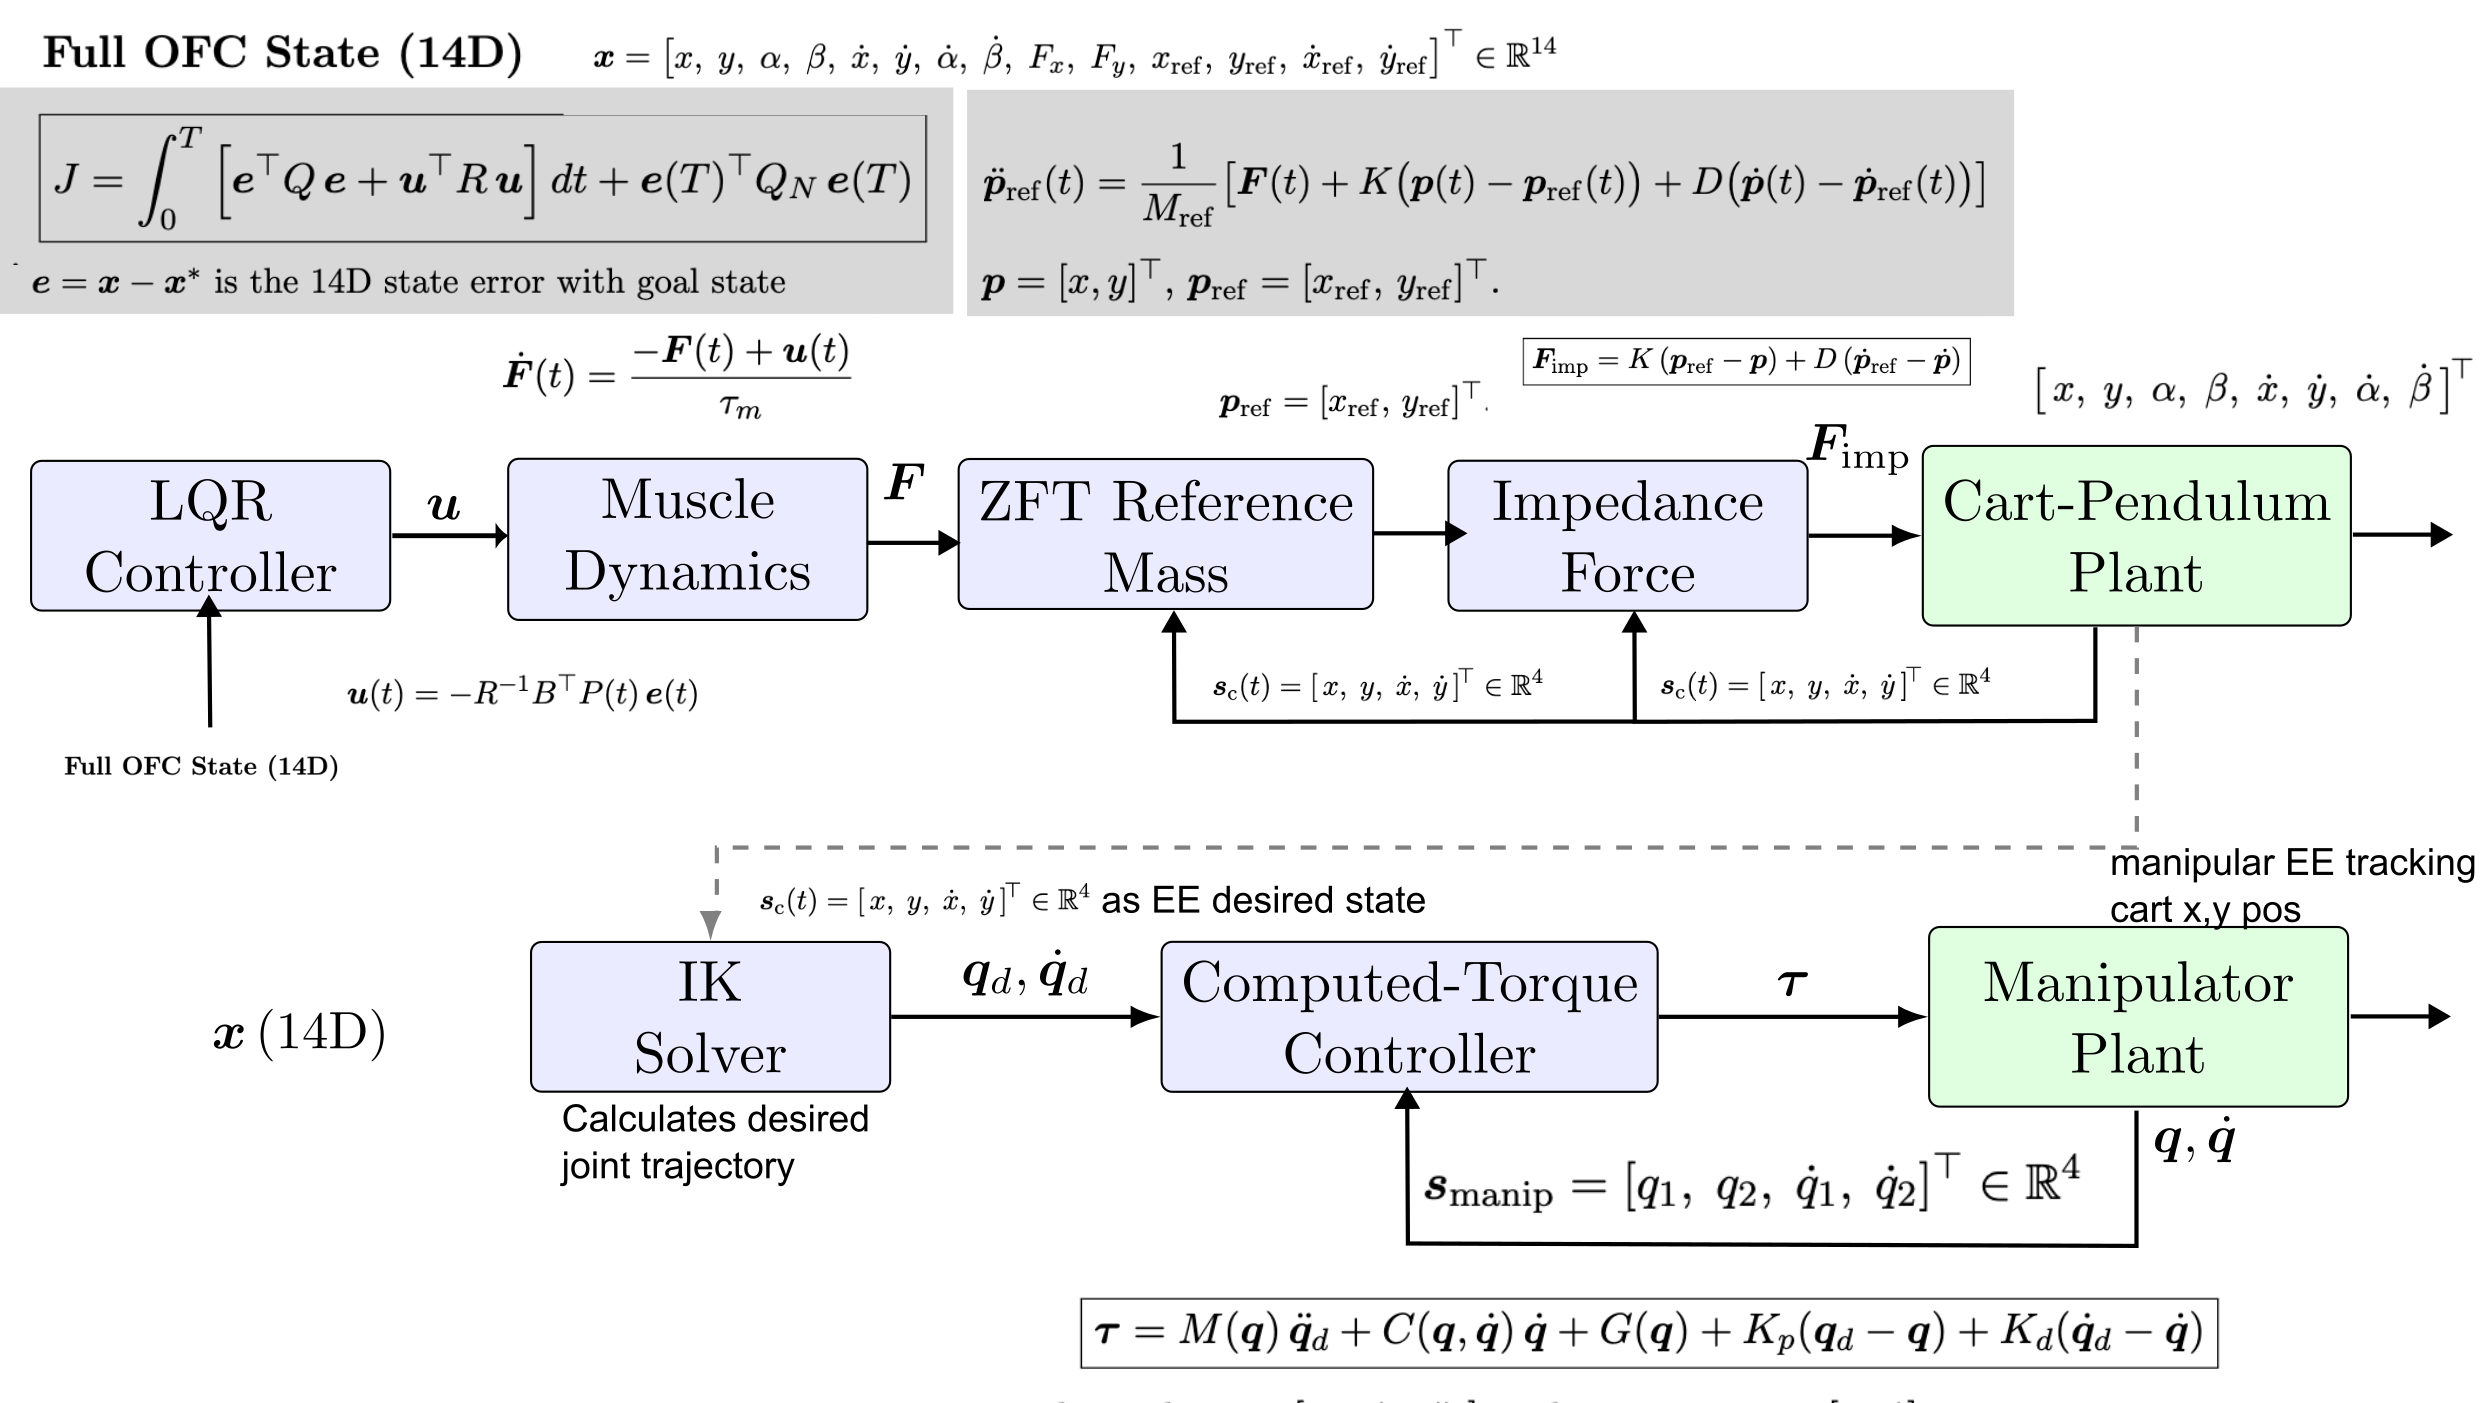
\includegraphics[width=\linewidth, height=0.85\textheight, keepaspectratio]{../notes_control/lqr_cart_manip_following.png}
\end{center}
\end{frame}

% ── Slide 7b: Cart-Pendulum OFC — Equations ─────────────────────────────────
\begin{frame}{Methodology: Cart-Pendulum OFC (14-D State)}
\begin{columns}[T]
  \column{0.48\textwidth}
  \textbf{Full OFC state:}
  \[
    \bm{x} = [x,y,\alpha,\beta,\dot x,\dot y,\dot\alpha,\dot\beta,
              F_x,F_y,x_r,y_r,\dot x_r,\dot y_r]^\top \in\mathbb{R}^{14}
  \]
  \textbf{Muscle dynamics} ($\tau_m = 30\,$ms):
  \[
    \dot{F}_i = \frac{-F_i + u_i}{\tau_m}
  \]
  \textbf{ZFT reference mass} ($M_\text{ref}=1\,$kg, $K=50$, $D=10$):
  \[
    M_\text{ref}\ddot{\bm{p}}_\text{ref}
      = \bm{F} + K(\bm{p}-\bm{p}_\text{ref}) + D(\dot{\bm{p}}-\dot{\bm{p}}_\text{ref})
  \]
  \textbf{Impedance force:}
  \[
    \bm{F}_\text{imp} = K(\bm{p}_\text{ref}-\bm{p}) + D(\dot{\bm{p}}_\text{ref}-\dot{\bm{p}})
  \]

  \column{0.48\textwidth}
  \textbf{Finite-horizon LQR cost:}
  \[
    J = \int_0^T \!\bigl[\bm{e}^\top Q\bm{e} + \bm{u}^\top R\bm{u}\bigr]dt
        + \bm{e}(T)^\top Q_N \bm{e}(T)
  \]
  \textbf{Backward Riccati:}
  \[
    -\dot{P} = A^\top P + PA - PBR^{-1}B^\top P + Q
  \]
  \textbf{Control law:}
  \[
    \bm{u}(t) = -R^{-1}B^\top P(t)\,\bm{e}(t)
  \]
  \vspace{4pt}
  \begin{block}{Cost matrices}
    \footnotesize
    $Q=\mathrm{diag}(100,100,500,500,10,10,100,100,0.1,0.1,1,1,0.1,0.1)$\\
    $Q_N = 2Q$, \quad $R = \mathrm{diag}(1,1)$
  \end{block}
\end{columns}
\end{frame}

% ── Slide 7c: Manipulator Control — Equations ───────────────────────────────
\begin{frame}{Methodology: Manipulator Tracking}
\begin{columns}[T]
  \column{0.50\textwidth}
  \textbf{Goal:} end-effector tracks cart position $\bm{p}_\text{cart}=[x,y]^\top$.\\[5pt]

  \textbf{IK Solver} (Drake \texttt{InverseKinematics}):
  \[
    f_\text{FK}(\bm{q}_d) = \bm{p}_\text{cart},
    \quad \|\bm{q}_d - \bm{q}_\text{prev}\|_2 \to \min
  \]
  Warm-started from previous solution for continuity.\\[6pt]

  \textbf{Computed-torque controller:}
  \[
    \bm{\tau} = M(\bm{q})\ddot{\bm{q}}_d
              + C(\bm{q},\dot{\bm{q}})\dot{\bm{q}}
              + G(\bm{q})
              + K_p(\bm{q}_d-\bm{q})
              + K_d(\dot{\bm{q}}_d-\dot{\bm{q}})
  \]

  \column{0.47\textwidth}
  \begin{block}{Manipulator state}
    $\bm{s}_\text{manip} = [q_1,q_2,\dot q_1,\dot q_2]^\top \in \mathbb{R}^4$
  \end{block}
  \vspace{5pt}
  \begin{block}{Implementation}
    \begin{itemize}\setlength\itemsep{2pt}
      \item Framework: PyDrake \texttt{MultibodyPlant}
      \item Linearisation: automatic Jacobian (Drake API)
      \item Both plants share one \texttt{DiagramBuilder}
      \item Simulation step: 1\,ms; horizon $T=10\,$s
      \item Visualisation: Meshcat 3-D (real-time)
    \end{itemize}
  \end{block}
\end{columns}
\end{frame}

% ── Slide 8: Simulation Results ─────────────────────────────────────────────
\begin{frame}{Our Implementation: Simulation Results}
\begin{center}
  \textbf{Finite-horizon LQR --- cup manipulator (EE tracking)}\\[4pt]
  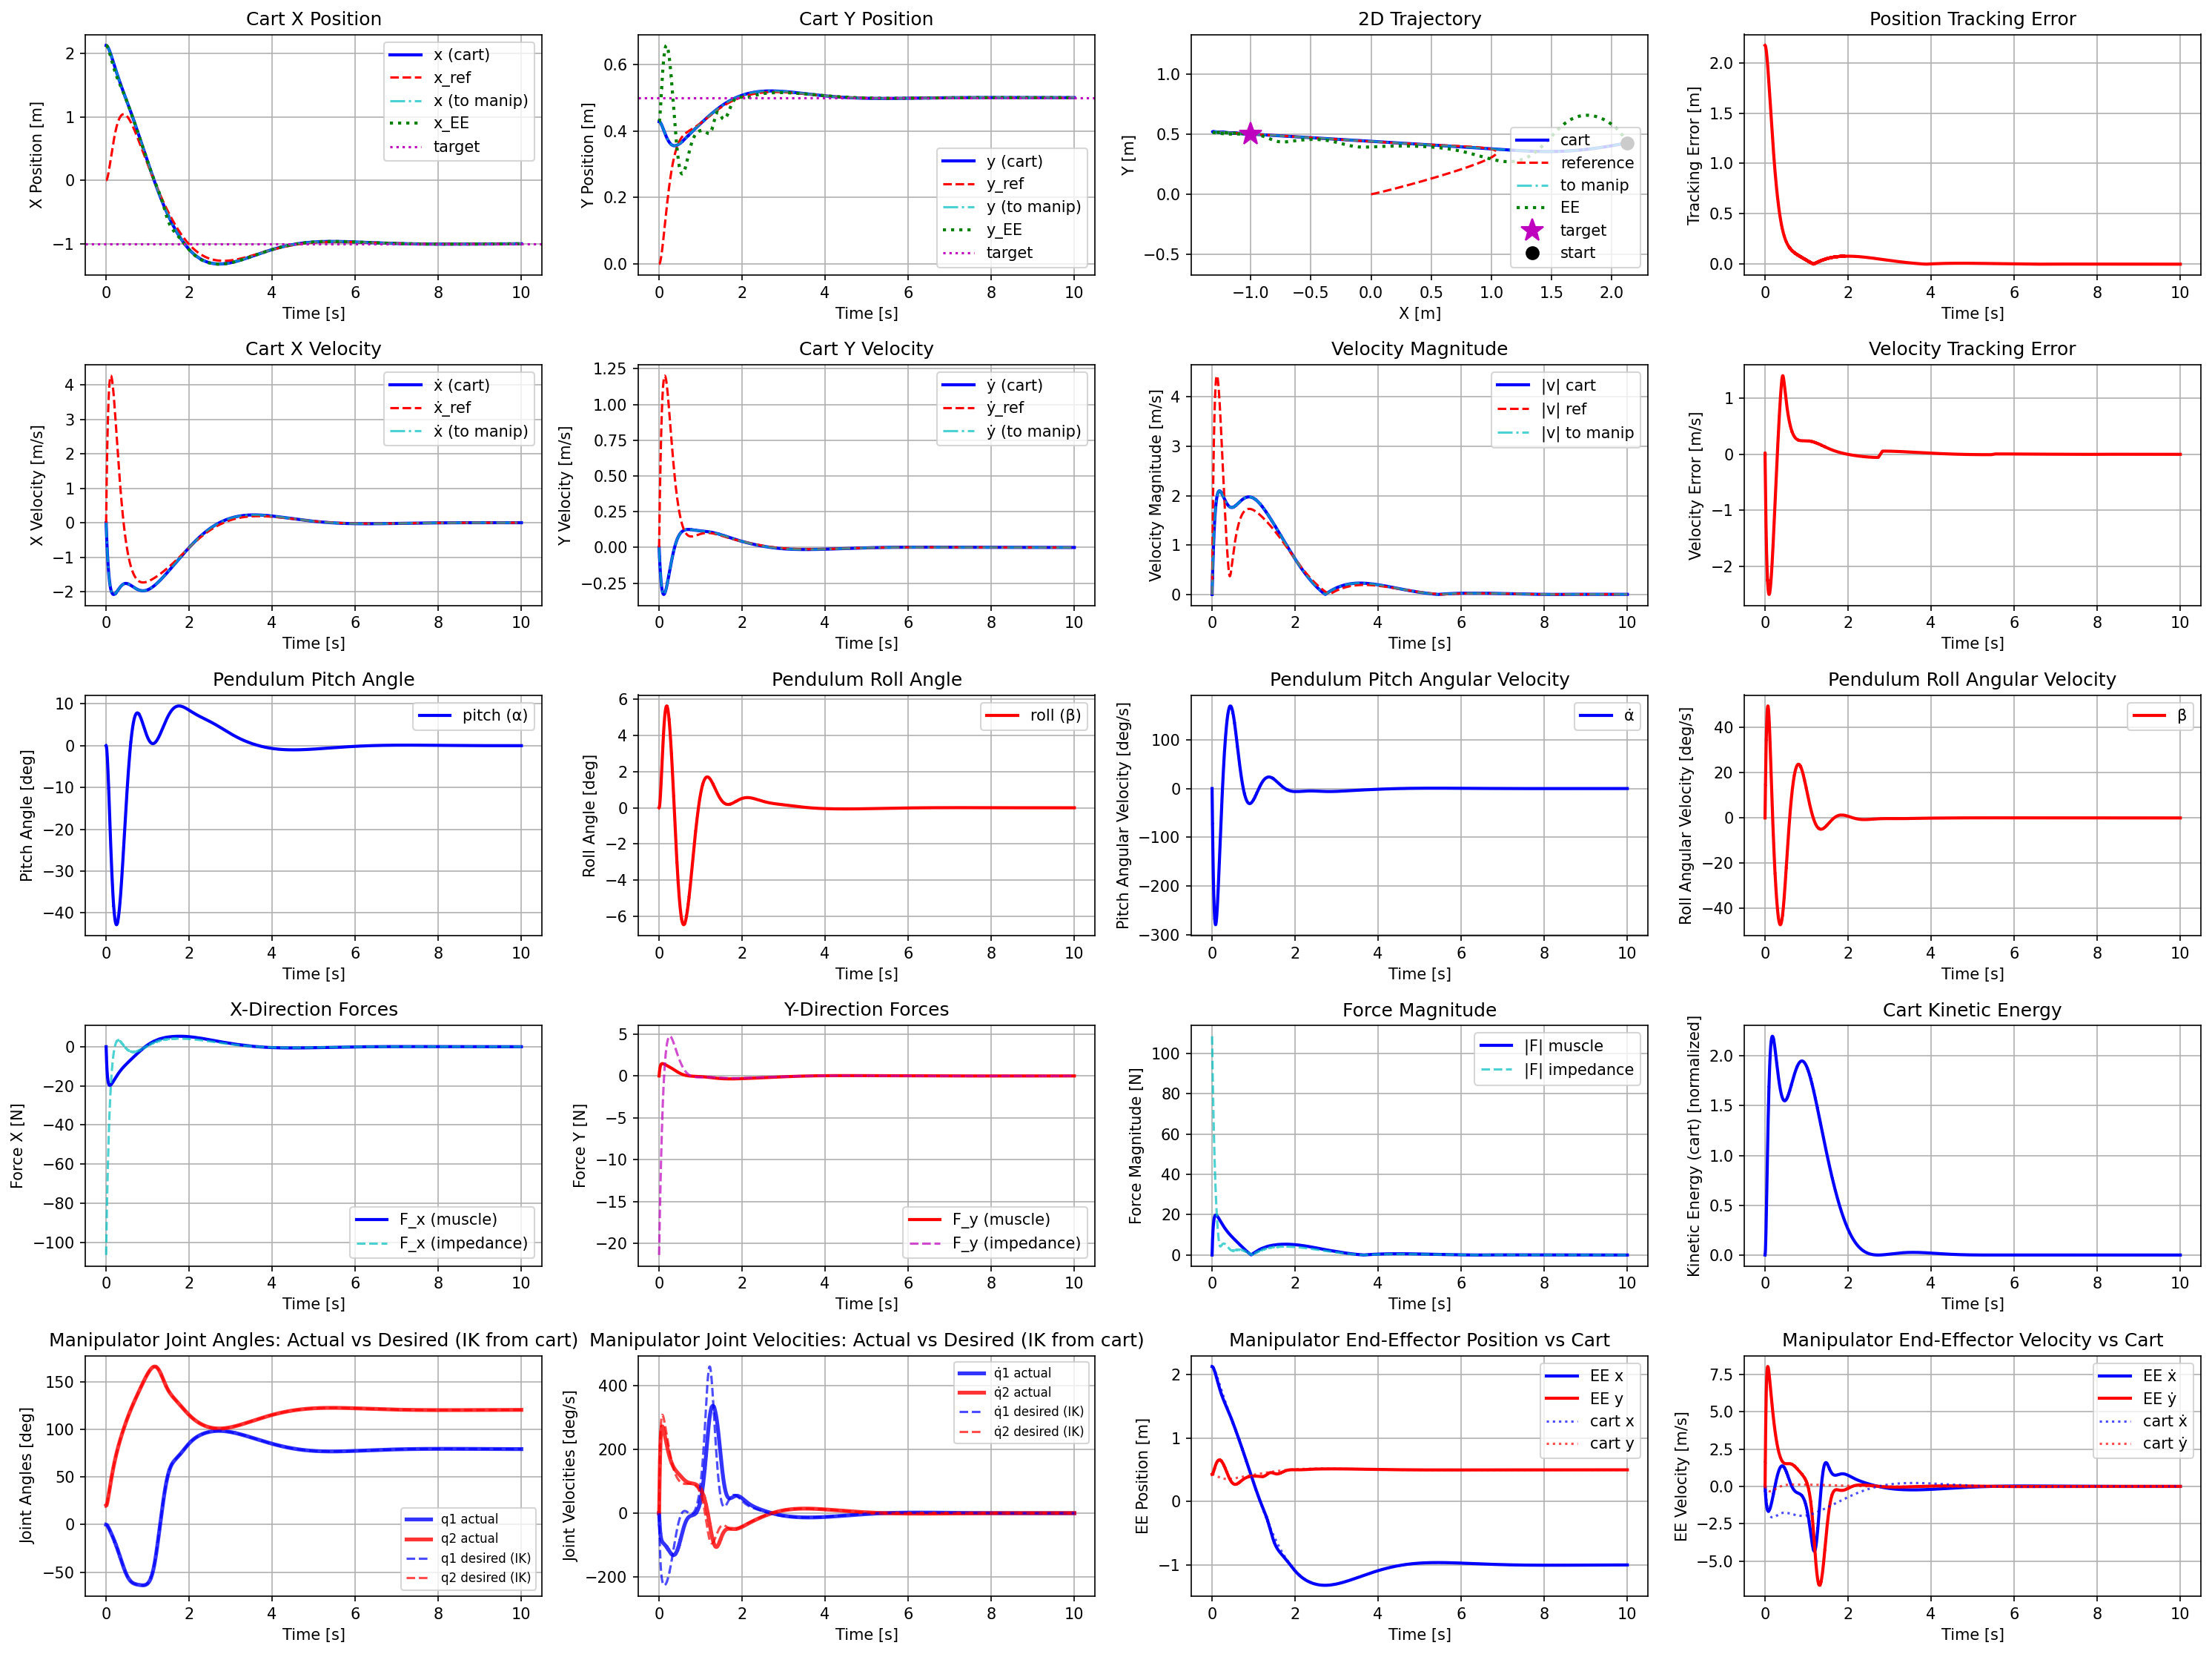
\includegraphics[width=\linewidth, height=0.8\textheight, keepaspectratio]{../plots/lqr_manip_ee_traj_track_results.png}
\end{center}
\vspace{2pt}

\end{frame}

\begin{frame}{Results Explanation}
    \begin{block}{Key observations}
  \begin{itemize}\setlength\itemsep{1pt}
    \item Cart reaches target position; pendulum angle stabilises to near-zero
    \item Muscle dynamics introduce a smooth ${\sim}90\,$ms force rise (3$\tau$) --- no torque spikes
    \item Impedance (ZFT reference mass) absorbs residual interaction forces without neural re-planning
    \item Manipulator end-effector follows cart via IK; joint torques remain within actuator limits
  \end{itemize}
\end{block}
\end{frame}

\end{document}
